\documentclass[12pt,letterpaper]{article}
\usepackage[latin1]{inputenc}
\usepackage[spanish]{babel}
\usepackage{amsmath}
\usepackage{amsfonts}
\usepackage{amssymb}
\usepackage{graphicx}
\usepackage[hidelinks]{hyperref}
\usepackage{color}
\graphicspath{{Imagenes/}}
\usepackage[left=2cm,right=2cm,top=2cm,bottom=2cm]{geometry}
\author{M�rquez M�rquez Amairani Ivette}

\begin{document}
\begin{center}
\textbf{\huge {Universidad Politecnica de la Zona \\[0.5cm] Metropolitana de Guadalajara}}
\end{center}

\begin{center}

\includegraphics[width=0.65\textwidth]{Imagenes/UPCDLZMDG5783-logo.png}\\[0.2cm] 
\end{center}
\vspace{0.1cm}
{\large\textbf{Evidencia:} 2.7 Dise�o de un Modulacion de Ancho de Pulso(PWM)con Amp-Op y transistores\\[0.2cm]\textbf{Alumna:} M�rquez M�rquez Amairani Ivette\\[0.2cm]\textbf{Profesor:} Mor�n Garabito Carlos Enrique\\[0.2cm]\textbf{Carrera:} Ing.Mecatronica\\[0.2cm]\textbf{Grupo:} 4�B\\[0.2cm]\textbf{Fecha de Entrega:} 22 de Octubre del 2019\\[0.2cm]}

\vspace{10cm}
\textbf{Ev. 2.7 Dise�o de un Modulaci�n de Ancho de Pulso(PWM)con Amp-Op y transistores}\\[0.2cm]

PWM(Modulador por ancho de pulso) es un dispositivo que puede usarse como un eficiente dimmer de luz o para controlar la velocidad en motores DC.\\
La funci�n que hay en un PWM es moderar o amplificar el periodo de las se�ales en el caso de los Amplificadores Operacionales se pueden hacer ciertas diferencias en las se�ales del ciclo util. Como se puede observa en la Figura 1. Amplificador - PWM 

 \begin{figure}[h]
\centering
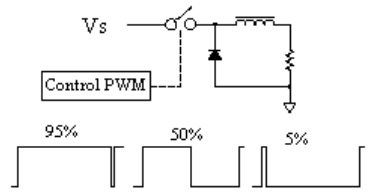
\includegraphics[width=0.50\textwidth]{Imagenes/1.PNG} 
\caption{Amplificador - PWM}
\label{fig:Motor}
 \end{figure}

En la figura 1 se muestra la operacion PWM mas simple.El bloqueo de control PWM convierte un nivel de entrada en una se�al de control con un ciclo util variante. Mientras mayor salida se requiera, el interruptor se mantiene encendido con una porci�n mayor del periodo.

\vspace{2cm}

 {\large\textbf{Bibliograf�a}\\[0.2cm]

  \emph{Romero.A(Junio del 2017). Base para el dise�o de amplificadores PWM.}
 Obtenido de:
 \textcolor{blue}{ https://revistas.udistrital.edu.co/index.php/Tecnura/article/download/6098/7622/}\\[0.3cm]
 
  \emph{Vidales.A(26 de Mayo del 2017). Modulador PWM por ancho de pulso.}
 Obtenido de:
 \textcolor{blue}{ https://issuu.com/sanchezdiaz/docs}\\[0.3cm]


\end{document}

